\documentclass[12pt]{article}
\pdfpagewidth 8.5in
\pdfpageheight 11.0in
\usepackage{fullpage}
\usepackage{url}
\usepackage{graphicx}
\usepackage{subfigure}
\usepackage{booktabs}
\usepackage{multirow}
\usepackage{rotating}
\usepackage{float}
\usepackage{acronym}
\usepackage{setspace}
\usepackage{amsmath}
\usepackage[hypcap]{caption}
\usepackage{hyperref}
\usepackage{tabularx}
\usepackage{bigstrut}
\usepackage{epstopdf}
%\onehalfspacing


\title{Deformable Mirror Demonstration}
\author{Kristin Berry\\
Ashley K. Carlton\\
Zachary J. Casas\\
James R. Clark\\
Vladimir Eremin\\ 
Zaira G. Garate\\ 
Julian Lemus\\
Immanuel David Madukauwa-David\\
Tam Nguyen T. Nguyen\\
Paul Salcido\\
Alexandra E. Wassenberg 
}

\date{\today}

\begin{document}
\maketitle
\newpage

\tableofcontents
\listoffigures
\listoftables


\section*{List of Acronyms}
\begin{acronym}

\acro{DeMi}{Deformable Mirror}

\end{acronym}
\newpage

%%%%%%%%%%%%%%%%%%%%%%%%%%%%%%%%%%%%%%%%%%%%%%%%%%%%%%
\section{Introduction}
		\subsection{Mission Statement}
		\subsection{Motivation}
\section{Mission Overview}
		\subsection{Requirements}
		\subsection{Concept of Operations -ZG}
		
		DeMi will be a 3-unit CubeSat on a low-Earth orbit with an altitude of 500 km at an inclination of 40°. Immediately separation from a standard Poly-PicoSatellite Orbital Deployer (P-POD), the satellite will begin to charge its primary batteries through solar panels covering the long faces of the structure. During this first stage, the satellite’s antenna will be deployed and will emit intermittent signals, or beacons, in order to be located by the ground station. The ADCS torque coils will detumble the satellite and align it in a nadir-pointing position. The detumble stage should last approximately 2 weeks. In case the satellite needs more time to power up, communicate with the ground station and stabilize itself, the science operations could be delayed. 
		
		\begin{figure}[!ht]
				\centering
				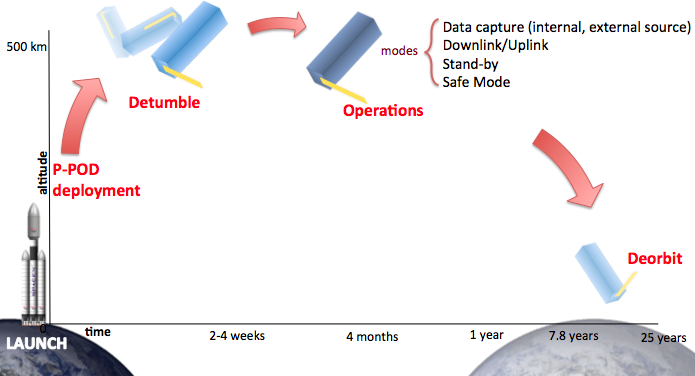
\includegraphics[width=5in]{images/MissionOverview_1.png}
				\caption{Timeline of the concept of operations for the DeMi Mission}
				\label{fig:Mission_ConOps}
			\end{figure}
		
		Once the satellite is in fully operational status, the payload will begin to conduct its scientific experiments and collect data. Two different data capture modes will be performed during the mission: internal source experiments will be done during the first 3 months of operations, while external source experiments will occur during the remainder of the mission. The satellite will attempt to downlink the collected data whenever it passes over the NASA Wallops ground station and is given instructions to begin downlink. 

The majority of the time, the satellite will be in stand-by mode; in other words, it will not be capturing or downlinking data. In case of a subsystem malfunction, the satellite will go into safe mode to diagnose the source of the problem. 

Analyses performed using STK predict that the satellite will deorbit within 7.8 years. This timeline agrees with the current 25-year deorbit requirement outlined by NASA standards.2

		\subsection{$N^2$ Diagram}
		
		In the early stages of the design process, the team created an $N^2$ diagram to exchange input and output values. Additionally, this diagram became an essential tool in determining the levels of interaction between the satellite’s different subsystems. 
		
		\begin{figure}[!ht]
				\centering
				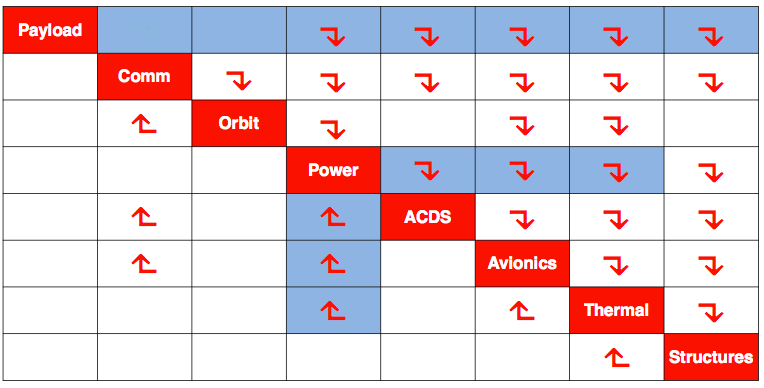
\includegraphics[width=5in]{images/MissionOverview_2.png}
				\caption{High-Level $N^2$ diagram showing input/output relationships between subsystems}
				\label{fig:Mission_N2}
			\end{figure}
			
		As highlighted the figure above, the payload requirements drive the design of all the other subsystems. While it does not receive design inputs from other subsystems, its design outputs cascade down effectively driving the design of the rest of the satellite. 

Feedback loops were present between several subsystems, which forced the team to perform trade studies to exchange performance for mass or power cost. One of these trades involved the design of the Power and ADCS subsystems. For example, complex solar panel designs that could absorb more solar energy, such as deployable panels, would require a more robust ADCS subsystem. However, such ADCS design would need to draw more power to maintain the panels facing towards the sun effectively cancelling the power gained. After careful consideration of costs and benefits, the team decided to take this option off the table
	
	\subsection{System Level Budgets}
		\subsubsection{Mass}
		The mass budget is presented in Figure~\ref{fig:Mission_mass2} below. 
			\begin{figure}[!ht]
				\centering
				\includegraphics[width=5in]{images/MissionOverview_3.png}
				%\caption{System Mass Budget}
				\label{fig:Mission_mass1}
			\end{figure}
		
			\begin{figure}[!ht]
				\centering
				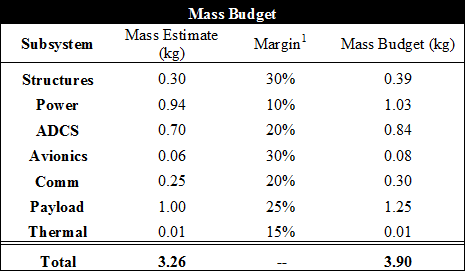
\includegraphics[width=5in]{images/MissionOverview_5.png}
				\caption{System Mass Budget}
				\label{fig:Mission_mass2}
			\end{figure}
			
		\subsubsection{Power}
		The power budget is presented in Figure~\ref{fig:Mission_power2} below. 
			\begin{figure}[!ht]
				\centering
				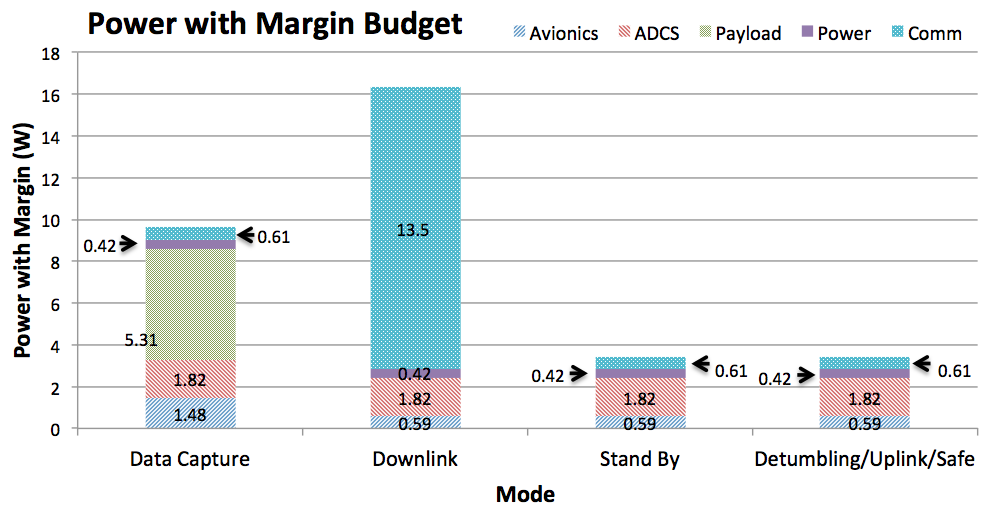
\includegraphics[width=5in]{images/MissionOverview_4.png}
				%\caption{System Power Budget}
				\label{fig:Mission_power1}
			\end{figure}
			
			\begin{figure}[!ht]
				\centering
				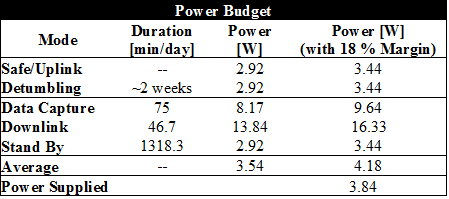
\includegraphics[width=5in]{images/MissionOverview_6.png}
				\caption{System Power Budget}
				\label{fig:Mission_power2}
			\end{figure}
			
\section{Subsystems}
		\subsection{Payload}
			\subsubsection{Requirements}
			\subsubsection{Trade Studies and Decisions Made}
			\subsubsection{Analysis}
			\subsubsection{Summary of Outputs}
			\subsubsection{Risks}
			\subsubsection{Future Work}
		\subsection{Power - JC}
			\subsubsection{Requirements}
			The Power subsystem is required to supply power to all other subsystems under all conditions.  In particular, it must supply an average of 3.54 watts on average over the course of the orbit (calculated in Section~\ref{subsubsec:power-analysis}, Analysis), sustain a maximum load of 13.84 watts during certain operational modes (downlink mode, per Systems), have a minimum battery capacity of 3.9 watt-hours (calculated in Section~\ref{subsubsec:power-analysis}, Analysis), and meet these requirements for up to 1 year, or approximately 6,000 cycles (calculated in Section~\ref{subsubsec:power-analysis}, Analysis).
			
			\subsubsection{Trade Studies and Decisions Made}
			Using STK, we compared the average power obtained by the solar panels under several circumstances.  The two variables were the inclusion or omission of a solar panel on the top face of the satellite, in addition to the four side-mounted panels, and the orientation of the satellite in its orbit -- whether it few ``face-first'', with the normal vector of one of its sides aligned with its velocity, ``corner-first'', where it is tilted by 45 degrees about its long axis from the face-first orientation, or spinning about its long axis.  The face-first and corner-first attitudes are illustrated below:
			
			\begin{figure}[ht]%
			\centering
			\includegraphics{images/power-face-first}%
			\hspace{0.5in}
			\includegraphics{images/power-corner-first}
			\caption{The ``face-first'' and ``corner-first'' attitudes.  Images generated from STK.}%
			\label{fig:power-face-first}%
			\end{figure}
			
			\begin{table}[ht]\label{table:power-trade-study}
\caption{Power values for various panel configurations and satellite attitudes.}
\begin{center}
    \begin{tabular}{|c|c|c|c|} \hline
    	 & Face-first & Spinning & Corner-first \\ \hline
Side panels & 3.77 W & 4.16 W & 4.52 W \\\hline
Side and top panels & 4.45 W & 4.84 W & 5.19 W \\\hline
    \end{tabular}
\end{center}
\end{table}

Note that these power values are averaged over the entire orbit -- that is, taking the incoming power to be zero during local night and including that in the average.  This was done because the satellite is active during the entire orbit, and its average power needs are calculated over the entire orbit; to ensure that we are comparing likes against likes, we did the same for the power generated.
			
			\subsubsection{Decisions Made}
			
			\begin{figure}%
			\centering
			\includegraphics[trim = 0 2cm 0 0, clip]{images/power-3U-side-paneled}%
			\caption{The solar panel configuration to be used on the DeMi satellite.  Image from Clyde Space.\cite{CS image}}%
			\label{fig:power-panels}%
			\end{figure}
			
In general, the power subsystem was designed to be as simple as possible while meeting the satellite's power needs.  We chose to use stock parts as much as possible because they have known performance, which helps us verify that requirements are met and reduces the margins we need to hold.

The chosen solar panel configuration was four body-mounted side panels.  Body-mounted panels were chosen over deployable panels because they minimized the surface area of the satellite, which minimized the disturbance torques, and they are symmetrical, reducing the pointing constraints on the ADCS.  The satellite would be oriented in a nadir-pointing configuration, so the nadir face would almost never see any sunlight, so we chose not to panel it, and we chose not to panel the zenith face to allow the payload to have an aperture in that face, so that it could potentially image external light sources.

The remainder of the power system is similar to that of most other satellites: an electrical power system module takes power from the solar panels and manages the current and voltage levels to ensure that the panels deliver power at maximum efficiency, a secondary (rechargeable) battery supplies the satellite with energy during eclipse, and a power distribution module supplies power to systems which are not part of the main system stack, like the torque coils.

The satellite's power subsystem does not include a primary battery.  A primary battery was never included in the design because the satellite was to be covered on most sides by solar panels and would be power-positive in detumbling mode, so it would charge as soon as it exited the P-POD.  The only reference to a Cubesat containing a primary battery was a description of a Cubesat that lacked solar panels entirely.\cite{libertad-1}
			
			\subsubsection{Analysis}\label{subsubsec:power-analysis}
			
The average power required is the time-weighted average of the power required during the various modes of the satellite:

\begin{equation}
P_{req,avg} = \frac{1}{T_{total}}\sum_{modes}{ \sum_{systems}{T_{mode} \: P_{sys,mode}} } = 3.54 \ \text{W} 
\label{eq:power-required}
\end{equation}

The solar panels are required to gather enough power during the day to power the satellite for the entire orbit, when taking the inefficiency of the EPS into account ($\eta = 0.85$ in the worst case\cite{EPS manual}):

\begin{equation}
P_{req,panels} = \frac{T_d + T_e}{T_d}\frac{P_{req,avg}}{\eta} = 6.61 \ \text{W (cold)}, 5.21 \ \text{W (hot)}, 4.16 \ \text{W (orbit avg)}
\label{eq:power-required-panels}
\end{equation}

``Hot'' and ``cold''\footnote{Perhaps ``bright'' and ``dark'' would be better terms from a power perspective, because it is not temperature that gives us power but sunlight.} here refer to the two orbital cases which have the most and least solar exposure for the satellite – because the orbit is fixed in inertial space, it appears to rotate with respect to the Earth-Sun vector over the course of a year.  Every six months, it goes from a “cold” orbit, which is in the sunlight 63\% of the time, to a “hot” orbit, which is 80\% sunlit, and back again.  The two orbits are illustrated below.

\begin{figure}[ht]%
\centering
\includegraphics{images/power-hot-orbit}%
\caption{A ``hot'' orbit, where the satellite is exposed to the sun 80\% of the time.  Image generated from STK.}%
\label{fig:power-hot-orbit}%
\end{figure}

\begin{figure}[ht]%
\centering
\includegraphics{images/power-cold-orbit}%
\caption{A ``cold'' orbit, where the satellite is exposed to the sun 63\% of the time.  Image generated from STK.}%
\label{fig:power-cold-orbit}%
\end{figure}

The satellite drains the most energy from the battery if it performs a ground station pass (maximum duration: 9.77 minutes, per Comm) and scientific operation (nominal duration: 5 minutes, per Payload) during local night:

\begin{equation}
E_{req,batt} = T_{sci} P_{sci} + T_{comm} P_{comm} + (T_e - T_{sci} - T_{comm}) P_{standby} = 3.9 \ \text{Wh}
\label{eq:power-batt-req}
\end{equation}

The excess power is the power actually generated by the panels that does not go into powering the satellite or charging the battery -- in other words, the difference between the power required power and the power actually generated:

\begin{equation}
P_{excess} = P_{panels} - P_{req,panels} = 0.63 \ \text{W (cold)}, 2.57 \ \text{W (hot)}
\label{eq:power-excess}
\end{equation}

It can be useful to model the excess power as an average over the entire orbit, rather than just happening during local day (for first-order approximations of the equilibrium satellite temperature):

\begin{equation}
P_{excess,avg} = P_{excess} \: \frac{T_d}{T_d + T_e} = 0.40 \ \text{W (cold)}, 2.06 \ \text{W (hot)}
\label{eq:power-excess-avg}
\end{equation}

The number of charge-discharge cycles of the battery is approximately equal to the number of orbits that the satellite will have to sustain:

\begin{equation}
N_{cycles} = \frac{T_{year}}{T_{orbit}} = 5500 \approx 6000 \ \text{(with 10\% margin)}
\label{eq:power-num-cycles}
\end{equation}

			\subsubsection{Summary of Outputs}

\begin{table}[ht]\label{table:power-outputs}
\caption{Outputs to other systems (mass, volume, power consumed, and survival and operating temperatures).\cite{EPS manual} \cite{PDM manual} \cite{Battery manual} \cite{Solar panel datasheet}}
\begin{center}
    \begin{tabular}{|l|l|l|p{0.8in}|p{1in}|p{1.1in}|} \hline
Component & Mass (kg) & Volume (U) & Power consumed (W) & Survival temperature ($^\circ$ C) & Operating temperature ($^\circ$ C) \\ \hline \hline
Solar panels & 0.540 & 0 & 0 & -40 to 80 & -40 to 80 \\\hline
EPS & 0.083 & 0.15 & 0.1 & -50 to 100 & -40 to 85 \\\hline
Battery & 0.256 & 0.2 & 0.1 & -10 to 50 & 0 to 50 \\\hline
PDM & 0.060 & 0.25 & 0.16 & -50 to 100 & -40 to 85 \\\hline \hline
Total & 0.939 & 0.6 & 0.36 & N/A & N/A \\\hline
    \end{tabular}
\end{center}
\end{table}

The solar panels do not literally have zero volume, but because they are fixed to the sides of the Cubesat, they do not occupy any of the three units of internal volume.

			\subsubsection{Risks}

The primary risk facing the Power subsystem is that our incoming power is fundamentally limited, so we will have to be careful to not exceed our budget.  As computed in Analysis (Section~\ref{subsubsec:power-analysis}), the average power drawn by the satellite for nominal mode durations is 3.54 watts.  While the orbit-averaged power coming in from the solar panels is 4.52 watts, which is a 28\% margin over the power needs, when we take the worst-case efficiency of the EPS's solar-panel connection into account\cite{EPS manual}, we find that as little as 3.84 watts are actually getting to the battery power bus, leaving only a 9\% margin (which might then be further eroded by inefficiencies in the power lines).  This is less than the 18\% margin goal we had set for ourselves, and substantially less than the 30\% margin that JPL informed us was their usual standard for satellite missions.

This risk is mitigated by the 32\% margin of available power over the standby power need of 2.91 watts.  From this, we can be confident that, even in the worst possible case, the satellite will be power-positive during its standby mode.  This means that, if the satellite should find itself unable to meet its power needs for nominal mode durations, it could be commanded to spend more time in standby mode and less in data capture or downlink mode to restore balance to its power budget.  As mentioned in the Analysis section, the available power was calculated for the coldest, darkest orbit that the satellite will be in.  For the brightest orbit, the average power generated by the solar panels over the entire orbit increases to 7.42 watts, which, taking the worst-case EPS efficiency into account, results in 6.31 watts reaching the power line, which is a 78\% margin over the average power required.  In fact, we could spend 29 minutes -- nearly six times the nominal data capture mode duration -- of such a bright orbit in data capture mode (leaving the downlink mode duration constant, as ground pass durations are independent of available power) while maintaining a 30\% margin of available (post-EPS) power over required power.  We can thus be assured that, even if the satellite is forced to reduce the duration of data capture and downlink modes during darker orbits to conserve power, we can make up for any shortfalls of captured data during better orbits.

			\subsubsection{Future Work}
The performance of the solar panels and batteries is temperature-dependent.  In particular, the battery becomes more effective as its temperature increases, while the solar panels become less so.  Going forward, it would be useful to perform a more detailed simulation of the satellite that incorporates a thermal model, so that we can more accurately measure the effect of satellite temperature and dissipated excess energy (energy from the solar panels that does not go into charging the battery or powering the satellite).
		
		\subsection{Communication}
			\subsubsection{Requirements - ZC}

Most of the Communications requirements (see Appendix~\ref{app:requirements}) are standard Communications requirements for operability. Comm-1 is simply stating what the main goal of the Communications subsystem is. Comm-2 is there to ensure that the link with the ground station is good enough to transmit all of the data that we need to. Comm-2.1 is there so that if there is an error in the transmission, the system will be able to realize this and ask for a correction. Comm-2.2 is so that it doesn’t try to downlink more data than possible because if it does, then data will be lost. Comm-3 is simply there so that the Communications subsystem can ensure access with the ground station. Comm-3.1 and Comm-3.2 are specifics when it comes to communicating with the ground station. Comm-4 is there because if we do not encrypt it, another satellite may be able to receive our commands and learn about the DeMi system. Comm-5 is there to ensure that if there are errors, there will be very few of them. Comm-6 is just to ensure that DeMi follows all regulations set by different government agencies.

			\subsubsection{Trade Studies - ZC}\label{sec:comm_tradestudies}
The main factor in choosing what transceiver to use in our system is the data downlink amount. Because payload is generating so much data, Communications will need to have a high downlink rate to ensure that all of that data can be sent to the ground. Several options were looked into, and shown in Table~\ref{table:comm_transceivers}.

\begin{table}[ht]
\caption{Communications Trade Study for Maximum Downlink Data Rate}
\label{table:comm_transceivers}
\begin{center}
    \begin{tabular}{| c | c |} \hline
    	Tranceiver & Maximum Downlink Rate \\ \hline \hline
Espace Payload Telemetry System & $1\ Mb/s$ \\
AstroDev Li-1 UHF Transceiver & $38.4\ kb/s$ \\
ISIS TXS Small Satellite  S-Band Transmitter & $100\ kb/s$ \\
Tyvak UHF Transceiver & $200\ kb/s$ \\
L-3 Cadet Nanosat UHF Radio & $1.5\ Mb/s$ \\
Microhard MHX2420 Modem & $230.4\ kb/s$ \\ \hline 
    \end{tabular}
\end{center}
\end{table}

			\subsubsection{Decisions Made - ZC}

Given the information in Section~\ref{sec:comm_tradestudies}, the L-3 Cadet Nanosat UHF Radio was chosen for use on DeMi. It will transmit at the frequencies and data rates outlined in the requirements, which are $445\ -\ 455\ MHz$ for uplink at $19.2\ kb/s$, $460\ -\ 470\ MHz$ for downlink at $1.5\ Mb/s$. The transceiver also has an extra $4\ GB$ of storage that avionics will be able to use in addition to any of its storage. 

\begin{figure}[ht]\label{fig:comm_Cadet}
\centering
  \includegraphics[width=3in]{images/comm-cadet.png}
\caption{Photo of the custom-designed high-speed L3 Cadet radio \cite{DICE}.}
\end{figure}

Because the transceiver will be transmitting and receiving at UHF frequencies, a very common antenna choice is to use a measuring tape antenna that is tuned to the frequency that is desired. Because the antenna works like a quarter-wave monopole, one can determine the desired length of the antenna by dividing the wavelength of the transmitted and received signal by 4. Because the transmitting and receiving frequencies are different, the average of these frequencies was used to compute the wavelength. 

\begin{equation}\label{eq:comm_lambda}
\lambda = c/f
\end{equation}

Eq.~\ref{eq:comm_lambda} is used to calculate the wavelength. $\lambda$ is the wavelength, $c$ is the speed of light, and $f$ is the frequency. Using the average frequency of $465\ MHz$, the wavelength equals $0.645\ m$. Then to determine the length of the antenna one can just use the following equation.

\begin{equation}\label{eq:comm_length}
l = \lambda/4
\end{equation}

In Eq.~\ref{eq:comm_length}, $l$ is the length of the antenna, and $\lambda$ is the wavelength. Using a wavelength of $0.645\ m$, one can find that the desired length of the antenna is about $0.164\ m$. The gain of this antenna will be approximately $3\ dB$ and the beam width approximately $65^\circ$.

\begin{figure}[ht]\label{fig:comm_tape}
\centering
  \includegraphics[width=3in]{images/comm-tape.png}
\caption{Photo of stored and deployed measuring tape antenna. The pictured CubeSat has four antennas. DeMi will only be using one \cite{antenna}.}
\end{figure}

The ground station that will be used with this system will be the NASA Wallops UHF Ground Station. This was chosen because the transceiver that will be used was also used in the Dynamic Ionosphere CubeSat Experiment, and the ground station that was used in that mission was the NASA Wallops UHF Ground Station. The diameter if the dish is $18.29\ m$, the gain is $35\ dB$ and the beam width is $2.9^\circ$.

			\subsubsection{Analysis - ZC}

One can calculate the maximum amount of data downlink per pass-by by multiplying the downlink data rate and the access duration per pass-by. Given the downlink data rate of $1.5\ Mb/s$, and the access duration of $586\ s$ per pass-by, the maximum amount of data that can be downlinked in one pass-by is $109.9\ MB$. To account for the fact that the data-rate won’t always be able to be at its maximum, and also for space for telemetry data and error correcting code, we have a margin of a factor of 2, so the maximum amount of data from payload that can be downlinked per pass-by is about $54.95\ MB$. Although this is not as much data as payload is creating, there will be on-board processing so that the amount of data that needs to be downlinked is below the maximum amount that is allotted for payload.

A Link Budget was created in order to determine the Link Margin for a worst case and a best case for uplink and downlink. Appendix~\ref{app:link_budgets} detail these budgets.

The first calculation in the Appendix~\ref{app:link_budgets} is to calculate the worst case propagation path length. We know that the best case length is $500\ km$ because that is the altitude at which the satellite is orbiting. Figure~\ref{fig:comm_angles} shows how a wave propagates through that atmosphere and will be explained beneath.

\begin{figure}[ht]
\centering
  \includegraphics[width=4in]{images/comm-angles.png}
\caption{Diagram of propagation path of a signal from a satellite \cite{ITU-R}.}
\label{fig:comm_angles}
\end{figure}

In order to determine the propagation path length, $r$, one must determine the path length of the first layer and the second layer and add them together. The equation for calculating \cite{ITU-R} the path length of a layer is as follows.

\begin{equation}\label{eq:path_length}
a_n = -r_n\cos(\beta_n) + \frac{1}{2}\sqrt{4r_n^2\cos^2(\beta_n)+8r_n\delta_n+4\delta_n^2} 
\end{equation}

In Eq.~\ref{eq:path_length}, $a_n$ is the path length through layer $n$, $r_n$ is the radii from the center of the Earth to the beginning of layer $n$, $\beta_n$ is the exiting incidence angle, and $\delta_n$ is the thickness of layer $n$.
The angle $\beta_n$ can be calculated \cite{ITU-R} using the following equation.

\begin{equation}\label{eq:betan1}
\beta_{n+1} = \arcsin\biggl(\frac{n_n}{n_{n+1}}\sin(a_n)\biggr) 
\end{equation}

In Eq.~\ref{eq:betan1}, $n_n$ is the refractive index of layer $n$, and $\alpha_n$ is the entry incidence angle. Angle $\alpha_n$ can be calculated with the last equation needed in order to calculate \cite{ITU-R} the propagation length.

\begin{equation}\label{eq:a_n}
a_n = \pi - \arccos \biggl(\frac{-a_n^2 - 2r_n\delta_n - \delta_n^2}{2a_n r_n + 2a_n \delta_n}\biggr) 
\end{equation}

Values that still need to be defined are $\beta_1$ (because it cannot be calculated using Eq.~\ref{eq:a_n}), $\delta_1$, $\delta_2$, $n_1$, and $n_2$. $\beta_1$ is just equal to the complimentary angle to the minimum angle at which the Wallops Ground Station can track, which is $5^\circ$. $\delta_1$ will be equal to the altitude at which the atmosphere ends which one can say is about $100\ km$. $\delta_2$ is just the orbiting altitude minus $\delta_1$. $n_1$, which is simple the refractive index of air, is $1.000293$. The last remaining value to be defined is $n_2$, which is the refractive index of a vacuum, which is just 1. Using these equations, one can find that $a_1$ equals $707\ km$, and $a_2$ equals $1375\ km$. This means that the worst case propagation path length is equal to $2082\ km$.

The next value calculated in the Link Budgets is the Equivalent, Isotropic Radiated Power (EIRP). In order to calculate the EIRP \cite{SMAD}, the following equation should be used.

\begin{equation}\label{eq:EIRP}
EIRP = P_{tx} + G_{tx} - L_{output} 
\end{equation}

In Eq.~\ref{eq:EIRP}, $P_{tx}$ is the transmitter power, $G_{tx}$ is the transmit antenna gain, and $L_{output}$ is the output loss which is equal to all losses associated with the transmitter. All of these values can be found in the Link Budget (Appendix~\ref{app:link_budgets}).

Another calculated value in the Link Budget is the Space Loss. This is the loss of the signal as it is transmitted through space. It can be calculated \cite{SMAD} using the following equation.

\begin{equation}\label{eq:L_s}
L_s = 92.45 + 20\log_{10}(r) + 20\log_{10}(f) 
\end{equation}

In Eq.~\ref{eq:L_s}, $L_s$ is space loss, $r$ is the propagation path length, and $f$ is the frequency of the transmitted signal. All of these values can also be found in the Link Budget (Appendix~\ref{app:link_budgets}.

The next equation can be used to calculate \cite{pozar} the transmitting antenna temperature.

\begin{equation}\label{eq:t_antenna}
T_{antenna} = \eta T_{sky} + (1 + \eta) \frac{T_{sky} + T_{ground}}{2} 
\end{equation}

In Eq.~\ref{eq:t_antenna}, $\eta$ is the antenna efficiency, $T_{sky}$ is the temperature of the space behind the receiving antenna. The temperatures used for uplink are determined by using the background temperature of space. For downlink, the temperature of the Earth is used. $T_{ground}$ is the temperature of the ground around the antenna. For uplink, this is the temperature of the Earth, and for Downlink, it is the background temperature of space.

The system noise temperature, $T_{sys}$, is calculated by adding the transmitting antenna temperature and the receiver temperature \cite{pozar}. The receiver temperature for both cases is unique to the receiver and can be determined by the manufacturer.

The next calculated value is the Receiver Gain to Noise Temperature. This is computed \cite{SMAD} using the following equation.

\begin{equation}\label{eq:G/T}
\frac{G}{T} =  G_{rx} - T_{sys} 
\end{equation}

In Eq.~\ref{eq:G/T}, $\frac{G}{T}$ is the Receiver Gain to Noise Temperature, $G_{rx}$ is the receiving antenna gain, and $T_{sys}$ is the system noise temperature. Using $\frac{G}{T}$, the total losses in the system, and EIRP one can determine \cite{SMAD} the Receiver Carrier to Noise Ratio.

\begin{equation}\label{eq:c/n}
\frac{C}{N_0} = EIRP + \frac{G}{T} - L_{total} + 228.6 
\end{equation}

Using that value and the data rate in decibels, one can calculate \cite{SMAD} the Energy per bit to Noise Ratio.

\begin{equation}\label{eq:eb/n}
\frac{E_b}{N_0} = \frac{C}{N_0} - R_b 
\end{equation}

Finally, the link margin can be determined by subtracting the required Energy per bit to Noise Ratio from the predicted one. 

\begin{figure}[ht]\label{fig:comm_best}
\centering
  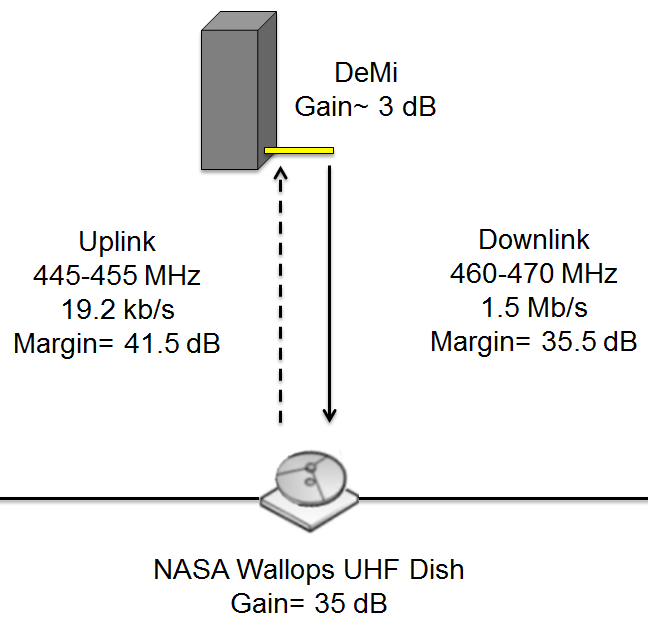
\includegraphics[width=4in]{images/comm-best.png}
\caption{Representation of Satellite and Ground Station during Best Case Communication.}
\end{figure}

\begin{figure}[ht]\label{fig:comm_worst}
\centering
  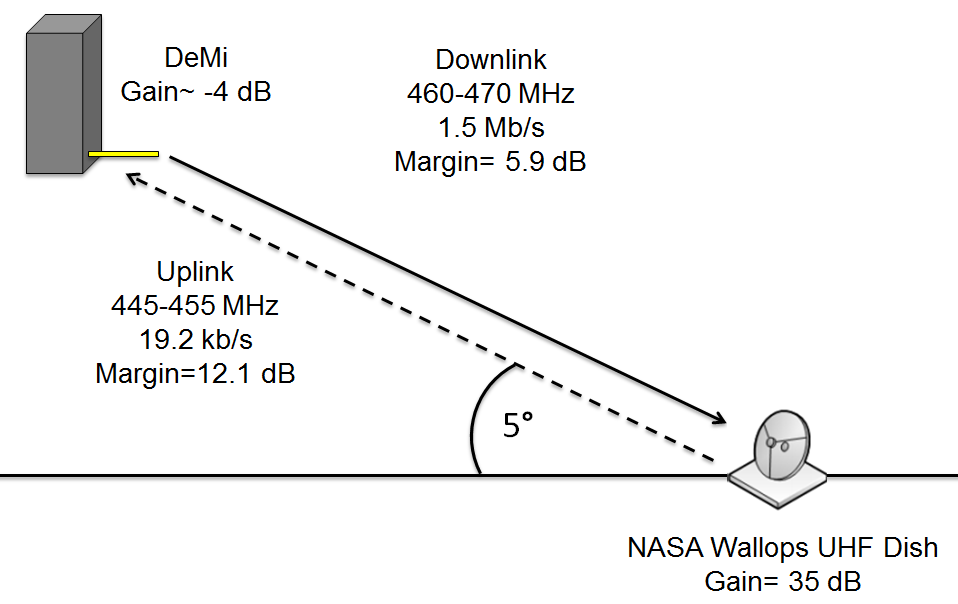
\includegraphics[width=4in]{images/comm-worst.png}
\caption{Representation of Satellite and Ground Station during Worst Case Communication.}
\end{figure}

			\subsubsection{Summary of Outputs - ZC}

There were several outputs during the design process from the Communications subsystem. These outputs include the Ground station to Orbits, which is NASA Wallops UHF Ground Station, the beam width of Wallops UHF Ground Station and DeMi to ADCS, which are $2.9^\circ$ and $65^\circ$ respectively, the operational and survival temperatures of the transceiver to Thermal, which are $-20^\circ$ C to $70^\circ$ C and $-40^\circ$ C to $80^\circ$ C respectively. The power for each mode to Power, and the mass and volume to Structures are detailed in Table~\ref{table:comm_summary_outputs}

\begin{table}[ht]
\caption{Communications Budgets}
\label{table:comm_summary_outputs}
\begin{center}
    \begin{tabular}{|c||c|} \hline
    	Output & Value \\ \hline \hline
    Power (Standby) & $0.51\ W$  \\
    Power (Data Capture) & $0.51\ W$ \\
    Power (Downlink) & $11.44\ W$ \\
    Power (Uplink) & $0.51\ W$ \\
    Power (Safe Mode) & $0.51\ W$ \\
    Mass & $0.235\ kg$  \\
    Volume & $0.069\ U$ \\ \hline 
    \end{tabular}
\end{center}
\end{table}

			\subsubsection{Risks - ZC}

As of PDR, there were no risks for the Communications subsystem. Towards the beginning of the design process, there were huge concerns about Communications not being able to downlink enough of the data from Payload, but since then, Avionics has decided that DeMi will be doing on-board processing so that all of the data does not need to be downlinked.

			\subsubsection{Future Work - ZC}

Moving on from here, the main thing that should be done is research and analysis of measuring tape antennas. There is currently not very much information out there that is available to DeMi concerning them, so research to determine the exact gain, beam width and radiation patterns should be conducted.		
		
		\subsection{Avionics}
			\subsubsection{Requirements - VE}
The Avionics subsystem requirements are presented in Appendix~\ref{app:requirements}.  The main driving requirements are number 3 and 2 in the order of importance because they are the most challenging to satisfy with a current level of technology.

			\subsubsection{Trade Studies - VE}
We have two main options that are able to satisfy the requirements for Avionics subsystem. Both are shown in Table~\ref{table:avionics_hardware_options}

\begin{table}[ht]
\caption{Hardware Options}
\label{table:avionics_hardware_options}
\begin{center}
    \begin{tabular}{| c || p{6cm} | p{6cm} |} \hline
     &	Processing on-board & Raw images to the ground \\ \hline \hline
    Component Name & The Steepest Ascent Mission Interface Computer CS-MIC-G-EM & Single Board Computer Motherboard + PPM with TI MSP430F2618 \\ \hline
    Power Consumption & $0.5\ -\ 1.25$ W & $10$ mW \\ \hline
    Capabilities & Telemetry/Telecommand + Real time image processing on FPGA & Telemetry/Telecommand\\ \hline
    Storage Capacity & Up to 16 GB & Up to 2 GB \\ \hline
    Processors & TI MSP430  + Xilinx FPGA (model can be selected) & TI MSP430F2618 \\ \hline
    Interfaces & I2C, SPI, UART & I2C, SPI, UART \\ \hline
    Mass & $62$ g & $88\ -\ 114$ g \\ \hline 
    \end{tabular}
\end{center}
\end{table}

Since we have identified the Payload driven requirements as the most challenging, we have to start selection of appropriate hardware from that.

\begin{table}[ht]
\caption{Payload image capturing modes}
\label{table:avionics_modes}
\begin{center}
    \begin{tabular}{| c || c | c | c |} \hline
    	Mode & 640x480 px subframe &  640x480 px subframe & 1280x1024 px  full frame \\ \hline \hline
    Frame Rate & $100\ fps$ & $10\ fps$ & $10\ fps$ \\
    Data Rate & $310\ Mbit/s$ & $31\ Mbit/s$ & $131\ Mbit/s$ \\
    Duration & $30\ s$ & $300\ s$ & $60\ s$ \\
    Memory Required & $1.14\ GB$ & $1.14\ GB$ & $0.96\ GB$ \\ \hline 
    \end{tabular}
\end{center}
\end{table}

Let’s consider approach when we downlink all the data generated by the Payload without processing it. From Table~\ref{table:avionics_modes} we can see that Payload will be generating around $1\ GB$ of data every time it is run. For a given $1.5\ Mbit/s$ downlink speed in this case we will need $600\ s$ to downlink all the data captured or 10 ground accesses. Since we have only one ground access every three orbits in general this particular approach seems to be too ineffective in terms of Payload active time. 

That’s why we mainly consider the second approach when we do all necessary calculations onboard and send only results to the ground. It dramatically reduces the amount of transferred data to around $10\ -\ 100\ KB$ instead of gigabytes and enables to implement a closed loop deformable mirror control system.

After we have solved a problem with data storage we can focus on the core of every Avionics subsystem - its processor. Now we have higher but still reasonable requirements for processing power according to the computation tasks that it will be solving: 1. Centroid, delta x and delta y, slope reconstruction, and 2. Linear algebra for mirror controller.
The Steepest Ascent Mission Interface Computer CS-MIC-G-EM is a good fit for such tasks because it has an FPGA to be configured for image processing and a microcontroller for general tasks such as telemetry and ADCS computations.

\subsubsection{Decisions Made - VE}

We have made a decision to use CS-MIC-G-EM (Figure~\ref{fig:avionics_MIC}) mainly because it enables onboard image processing which reduces the amount of data we send to the ground and provides with a capability to build a closed loop deformable mirror control system.

\begin{figure}[ht]
\centering
  \includegraphics[width=4in]{images/avionics-MIC.jpg}
\caption{Mission Interface Computer CS-MIC-G-EM \cite{avionics_clyde_space}}
\label{fig:avionics_MIC}
\end{figure}

It is also capable of providing the following interfaces with other subsystems see Table~\ref{table:avionics_interfaces}.

\begin{table}[ht]
\caption{Avionics hardware interfaces with other subsystems (*assuming update 10 times per second).}
\label{table:avionics_interfaces}
\begin{center}
    \begin{tabular}{| c | c | c | c |} \hline
    	Subsytem & Component & Interface & Data rate \\ \hline \hline
    Payload & Detector (IDS UI-5241LE-M) & GbE & $550\ Mbit/s$ max  \\
     & Mirror driver (BMC Mini-Driver) & USB 2.0 & $480\ Mbit/s$ max \\
     & Laser (ThorLabs CPS 186) & GPIO & -- \\ \hline
    Power & EPS, PDM & 12C & $400\ Kbit/s$ max \\ \hline
    ADCS & 5 sun sensors & analog & $100\ bit/s$* \\
     & ADIS16305 IMU/Magnetometer & SPI & $160\ bit/s$* \\
     & Torque coils & 12C (via PDM) & -- \\ \hline
    Thermal & 14 Temperature Sensors & analog & $100\ bit/s$* \\
     & Thermal Heater & 12C (via PDM) & -- \\ \hline
    Communication & Cadet NanoSat UHF Radio & RS232 & $1.5\ Mbit/s$ \\ \hline 
    \end{tabular}
\end{center}
\end{table}

			\subsubsection{Analysis - VE}
The system architecture in general is shown in Figure~\ref{fig:avionics_architecture}. The Mission Interface Computer we have selected allows us to separate telemetry from image processing data. The first is processed on CPU while the latter is done on FPGA.

\begin{figure}[ht]
\centering
  \includegraphics[width=7in]{images/avionics-architecture.jpg}
\caption{Caption goes here...}
\label{fig:avionics_architecture}
\end{figure}

			\subsubsection{Summary of Outputs - ZC}
The Avionics system had very few outputs to the other subsystems. It had to give values to Thermal for operational temperature range for the computer which is $-25^\circ$C to $85^\circ$C. The survival temperature is unknown. It also had to give outputs to power for power consumed during the different modes, and to structures for the mass and volume. These outputs, or budgets are detailed in Table~\ref{table:avionics_summary_outputs}.

\begin{table}[ht]
\caption{This is a summary of the mass totals, power needs, and thermal needs of the avionics system.}
\label{table:avionics_summary_outputs}
\begin{center}
    \begin{tabular}{|c||c|} \hline
    	Output & Value \\ \hline \hline
    Power (Standby) & $0.5\ W$  \\
    Power (Data Capture) & $1.25\ W$ \\
    Power (Downlink/Uplink) & $0.5\ W$ \\
    Power (Safe Mode) & $0.5\ W$ \\
    Mass & $0.062\ kg$  \\
    Volume & $0.104\ U$ \\ \hline 
    \end{tabular}
\end{center}
\end{table}

			\subsubsection{Risks - ZC}
There are two risks that avionics faces currently. One risk which is a high consequence, but a very low likelihood is that the system will not be capable of processing all of the incoming data for payload. Payload is outputting a lot of data, and because the design of the code that will do the process has not yet been done, it is unclear how quickly Avionics will be able to process incoming data. The other risk that Avionics is currently faces, which is of very low likelihood, but very high consequence, is that it will not be capable of providing the required latency for Payload or for ADCS. Research needs to be conducted to determine how fast avionics can receive and issue orders to ensure that the computer is fast enough for the system. If it is not fast enough there could be major failures in the system because the attitude of the craft is not correct.

			\subsubsection{Future Work - ZC}
The future work that needs to be conducted is that there should be work done to determine a new solution to interfacing with Payload. The mirror driver interfaces with USB 2.0, however the computer is not able to interface with this. So work should be done into determining how to resolve this. One other thing that should be looked into is ensuring that the system can run all of the necessary calculations at the required speed so that all of the payload data can be processed and sent to the ground. If all of the data can’t be processed, it would be difficult to complete our science goals.

		%%%%%%%%%%%%%%%%%%%%%%%%%%%%%%%%%%%%%%%%%%%%%%%%%%%%%%%%%%%%%%%%%%%%%%%%%%%%%%%%%%%%%%%%%%%%%%%%%%%%%%%%%%%%%%%%%%%%%%%%%%%%%%%%%%%%%%%%%%%%%%%%%%%%%%%%
		\subsection{Attitude Determination and Control System (ADCS) - TN} 
		%%%%%%%%%%%%%%%%%%%%%%%%%%%%%%%%%%%%%%%%%%%%%%%%%%%%%%%%%
			\subsubsection{Requirements}
		
				The two main driving requirements for the ADCS subsystems are the 			pointing requirement (15$^o$) for communication purpose and the stability requirement (0.08$^o$/s) for the payload operation while imaging an external source. Another requirement is the time for the satellite to detumble and establish ground station access before starting operation modes. This duration is required to be less than 30 days, creating a secondary requirement on the total detumbling time, which is dependent of the ADCS system. 
		%%%%%%%%%%%%%%%%%%%%%%%%%%%%%%%%%%%%%%%%%%%%%%%%%%%5
			\subsubsection{Trade Studies}
			Several control methods were considered in the design process of the ADCS system: passive magnetic control, passive magnetic control, and control using reaction wheels. The main trades to be considered are mass, power usage, pointing accuracy, and pointing stability capability. 

In passive magnetic control, restoring torque is generated through the alignment of the satellite magnetic moment with the local geomagnetic field. The magnetic moment is created through the use of permanent magnets. Hysteresis rods are used for vibration damping. This control option requires low mass and no power. Based on past CubeSat missions, the pointing accuracy of a passive magnetic control system in the same scale as DeMi can achieve 10 – 20 $^o$ [SMAD, cubesat survey], sufficient for communication requirement purpose. However, there are limitations in the ability to stabilize the satellite. Passive magnetic control systems stability performance is not reliable as the hysteresis rods do not provide fast and robust vibration damping. The expected stability achieved by this method is $1^o – 10 ^o$/s [cubesat survey]. Since the satellite will only have access to the external sources for a short amount of time, this method is not practical for capturing light from the stars. In addition, this control method limits the possible orientation of the satellite to only the direction along the local magnetic field. In a LEO orbit of 40$^o$ inclination such as that of DeMi’s, the direction of the local magnetic field varies at different orbital parameters, causing difficulties in placing antenna and external source aperture so that ground station access and external source capture can be guaranteed. 

Reaction wheels provide robust 3-axis stabilization control of the satellite. This control mechanism provides high accuracy ($~ 0.0001^o – 1^o$) in pointing direction and quick response in vibration damping providing high stability (0.05$^o$/s). However, the necessary sensors and actuators require high mass and power usage. The main mass contribution and power draw are from the reaction wheels. In addition, magnet torquers are also needed to desaturate reaction wheels, adding more mass and power strain on the system. This option is not practical for a small satellite such as DeMi. 

Active magnetic control was chosen for this mission due to the low mass and low power requirement and sufficient attitude control performance for both communication requirement and payload science operation. According to documentation on the attitude control system of the 1U CubeSat COMPASS-1 from the Univesity of Applied Sciences, Aachen, Germany, 3 magnetic coils of magnetic moment of  0.097 $A \cdot m^2$ can achieve a pointing accuracy of 8$^o$[reference]. The torque coils can be sized to generate enough torque for a 3U CubeSat. The details of this calculation will be presented in the decision made and analysis section. The stability of this control method is estimated to be $< 0.12^o$/s, according to the ION 2U CubeSat from the University of Illinois [ref.]. The implementation of the active magnetic control the ION mission only includes magnetometer as sensor with low magnetic moment in each torque coils. The performance of the active magnetic control method is expected to improve significantly with the use of more accurate sensors, such as an IMU and sun sensors, and torque coils with higher magnetic moment. More analysis and testing will be needed to determine the stability of the system. 
			\subsubsection{Decision Made}
				\paragraph{Orientation}
				The satellite will be in nadir pointing orientation with the nadir face being one of the two 10 cm x 10 cm faces. This orientation can be easily achieved by active magnetic control through sending control commands based on sensors readings to the active actuators. The 3U structure of the satellite provides gravity-gradient stability along the long axis in the nadir pointing configuration. By placing an antenna on the nadir face, this orientation facilitates access to the ground station. The satellite will travel with a corner-first configuration, to optimize the amount of power acquired from solar panels (see power section for more details). The orientation of the satellite is illustrated in Figure~\ref{fig:ADCS_orientation} below. 
			
			\begin{figure}[!h]
				\centering
				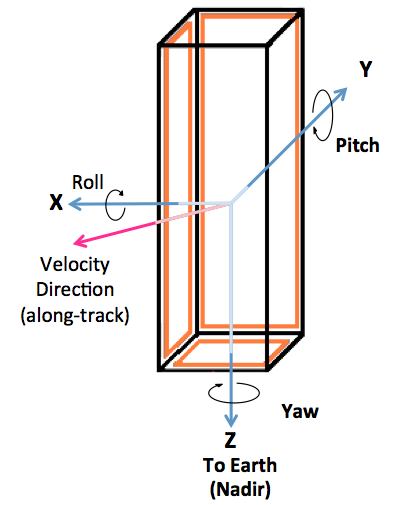
\includegraphics[scale=0.7]{images/ADCS_coord.png}
				\caption{Satellite orientation with respect to nadir direction and velocity vector}
				\label{fig:ADCS_orientation}
			\end{figure}
				
				\paragraph{ADCS sensors and actuators}
				A summary of the sensors and actuators used in the ADCS is presented in Table~\ref{tab:ADCS_sensors} below. 
			% Table generated by Excel2LaTeX from sheet 'Sheet1'
\begin{table}[htbp]
  \centering
  \caption{ADCS Sensors and Actuators}
    \begin{tabular}{|r|r|r|r|r|}
    \hline
    Sensors/Actuators & Quantity & Vendor & Performance &  \bigstrut\\
    \hline
    Sun sensors & 5     & CubeSat shop & \multicolumn{1}{r}{- Field of view: 114$^o$} &  \bigstrut[t]\\
          &       &       & \multicolumn{1}{r}{- Accuracy: $< 0.5^o$} &  \bigstrut[b]\\
    \hline
    Magnetometer & 1     & Analog Devices  & \multicolumn{1}{r}{- Dynamic range: ± 3.5 gauss} &  \bigstrut[t]\\
          &       & (ADIS16405) & \multicolumn{1}{r}{- Initial bias: ± 4 mgauss} &  \bigstrut[b]\\
    \hline
    IMU   & 1     & Analog Devices  & \multicolumn{1}{r}{- Dynamic range: ±300$^o$/s} &  \bigstrut[t]\\
          &       & (ADIS16405) & \multicolumn{1}{r}{- Initial bias: 3$^o$/s} &  \\
          &       &       & \multicolumn{1}{r}{- In-run bias stability: 0.007$^o$/s} &  \bigstrut[b]\\
    \hline
    Torque coils & 3     & N/A   & \multicolumn{1}{r}{- Max magnetic moment: 0.060, 0.063 $Am^2$} &  \bigstrut\\
    \hline
    \end{tabular}%
  \label{tab:ADCS_sensors}%
\end{table}%

			For attitude knowledge, a combination of sensors was chosen: sun sensors, magnetometers, and IMU.  The sun sensors are low mass and low power attitude sensors that provides accurate sun angle during day time, providing the orientation of the satellite relative to an inertial frame. 5 sun sensors will be places on the faces of the satellite other than the nadir face. This sensor, from CubeSat shop provides an accuracy of $< 0.5^o$ and a wide field of view of 114$^o$. The magnetometer will be used to measure the local geomagnetic field to compute the magnetic moment needed to generate needed restoring torques. In addition, the magnetometer will be used as the main attitude sensing device during eclipse periods. An IMU is used to measure the angular rate of the satellite to provide more accurate vibration knowledge to yield a robust vibration damping control loop. The IMU and magnetometer are in the same sensor unit from Analog devices. Both sensors have initial biases that can be corrected through computation. 

For actuation, 3 custom-made orthogonal torque coils will be used for 3-axis stabilization control. The coils will be sized so to meet the mass and power constraint of the satellite and to provide sufficient magnetic moment to counter environmental disturbances. More detailed calculation will be presented in the analysis section. The specifications of the torque coils are presented in Table~\ref{tab:ADCS_torquecoils} below.
			% Table generated by Excel2LaTeX from sheet 'Sheet2'
\begin{table}[htbp]
  \centering
  \caption{Torque coils specifications}
    \begin{tabular}{|r|r|r|}
    \hline
    Direction & Z     & X, Y \bigstrut\\
    \hline
    Size  & 10 cm × 10 cm  & 10 cm x 30 cm \bigstrut\\
    \hline
    Quantity & 1     & 2 \bigstrut\\
    \hline
    Turns & 500   & 300 \bigstrut\\
    \hline
    Current & 0.12 A & 0.07A \bigstrut\\
    \hline
    Wire Gauge & 28 AWG & 28 AWG \bigstrut\\
    \hline
    Magnetic moment & 0.60 $Am^2$ & 0.63 $Am^2$ \bigstrut\\
    \hline
    \end{tabular}%
  \label{tab:ADCS_torquecoils}%
\end{table}%
				\paragraph{System Schematics and Interfaces}
				The system schematics are shown in Figure~\ref{fig:ADCS_schem}. The IMU/magnetometer unit, which will be mounted on an interface board, and the sun sensors will be read out through the analog channels of the power distribution module. The module will be used as an interface to the avionics subsystem. The attitude knowledge data will be processed in the avionics subsystem. Combining with the local magnetic field, the magnetic moment vector needed for the torque coils can be computed. This information will be sent to the torque coils through the Power Distribution Module (PDM), into the torque coil driver, which consist of a current driver and an H-bridge, which controls the current in each coils and their directions. 
			
			\begin{figure}[!ht]
				\centering
				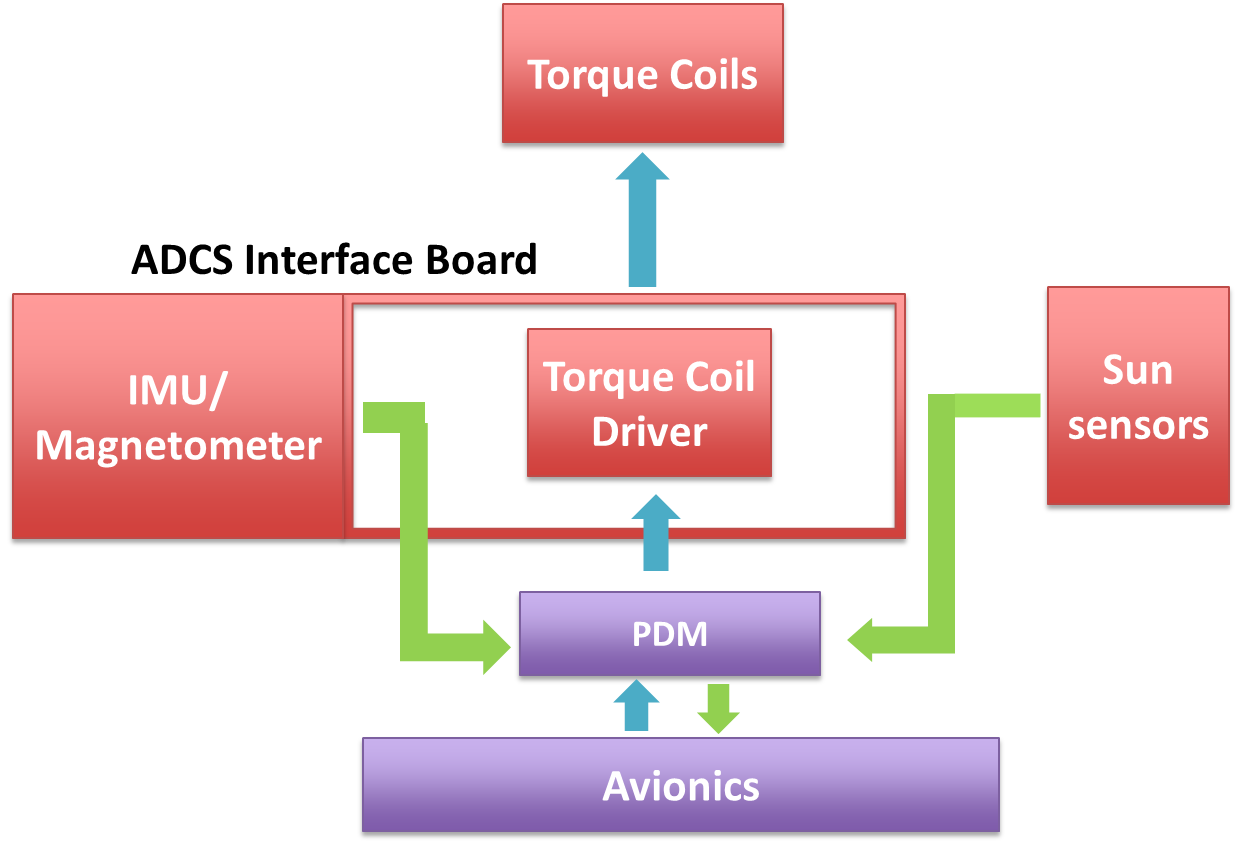
\includegraphics[scale=0.5]{images/ADCS_schem.png}
				\caption{ADCS components interactions and Avionics interface}
				\label{fig:ADCS_schem}
			\end{figure}
			
			\subsubsection{Analysis}
				\paragraph{Environmental Torque Calculation}
				The main environmental disturbances on orbit are gravity gradient, magnetic field, aerodynamics drag, and solar radiation pressure. The governing equations of these external sources are presented in details in SMAD ADCS section. Using the satellite properties, these values can be computed and presented in Table~\ref{tab:ADCS_envtorque}. 
				
				% Table generated by Excel2LaTeX from sheet 'Sheet3'
\begin{table}[htbp!]
  \centering
  \caption{Maximum Environmental Torque Estimation}
    \begin{tabular}{|r|r|}
    \hline
    Gravity Gradient & 1.60E-08 Nm \bigstrut\\
    \hline
    Magnetic Field & 1.80E-05 Nm \bigstrut\\
    \hline
    Atmospheric Drag & 2.70E-07 Nm \bigstrut\\
    \hline
    Solar Pressure & 5.50E-09 Nm \bigstrut\\
    \hline
    Total Torque & 1.80E-05 Nm \bigstrut\\
    \hline
    \end{tabular}%
  \label{tab:ADCS_envtorque}%
\end{table}%

			\paragraph{Torque coil sizing calculation}
			Magnetic control relies on the torque provided by the aligning of the satellite magnetic moment and the local magnetic field. Equation~\ref{eqn:ADCS_torque} shows the governing equation of magnetic control, where $\vec{T}$ represent the generated torque vector, $\vec{\mu}$ is the satellite magnetic moment, $\vec{B}$ is the local geomagnetic field vector. 
			
			\begin{equation}
				\vec{T} = \vec{\mu} \times \vec{B}
				\label{eqn:ADCS_torque}
			\end{equation}
			
			Taking the torque vector to be the total environmental torque, Equation~\ref{eqn:ADCS_torque} above yields the required maximum magnetic moment of the coils to be $~ 0.6 Am^2$. Since the area of each coil is chosen to be the same as the size of each of the face of the satellite, the main trade of the design is the number of turns and current in each coil. This corresponds to a mass/power trade. The results of the torque coil sizing are presented above in Table~\ref{tab:ADCS_torquecoils} in Decision Made section. 
			
			\paragraph{Detumbling Analysis}
				Using Princeton Satellite Systems MATLAB simulation, the momentum unloading as a response to an initial angular rate can be computed. The input parameters are the magnitude and direction of initial angular momentum, the direction of magnetic moment, and the gain of the control loop. The initial momentum was calculated by assuming an initial angular rate. The magnetic moment direction is the direction of the torque coils. The control gain is adjusted so that the maximum magnetic moments along all 3 axes are less than the maximum magnetic moments provided by the torque coils. The detumbling time can be calculated through determining the time where the momentum in all direction is less than an arbitrary low threshold. 

The simulation was run with an initial angular rate of 10$^o$/s, magnetic moment along x, y, z and a control gain of $k =0.008$. The angular momenta and magnetic moments are presented in Figure~\ref{fig:ADCS_detumbling}.
			
			\begin{figure}[!ht]
				\centering
				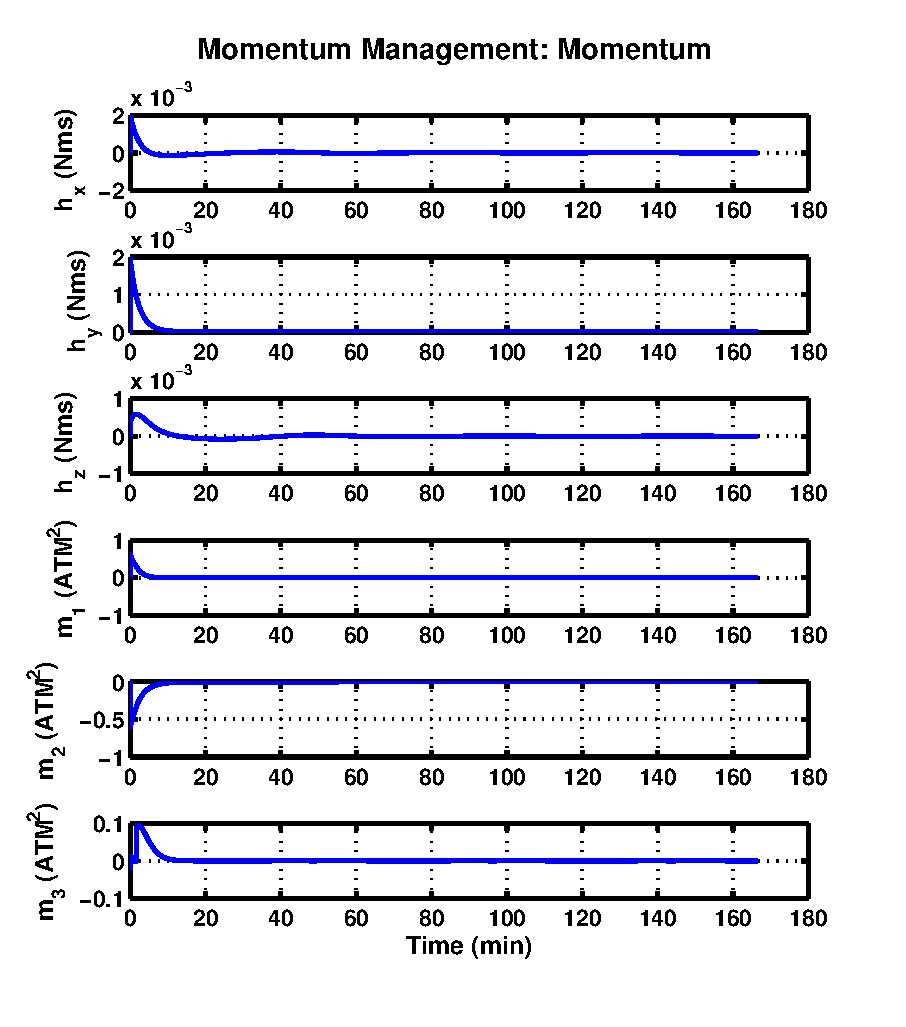
\includegraphics[scale=0.8]{images/ADCS_detumbling.eps}
				\caption{Momentum and magnetic moment during detumbling period}
				\label{fig:ADCS_detumbling}
			\end{figure}

			The maximum magnetic moment needed in x, y, z are 0.6092 $Am^2$ , 0.6052 $Am^2$, 0.0938 $Am^2$, respectively, which is within the range of magnetic moment the torque coils can provide. The total detumbling time is less than 1 orbit (90 minutes). 
			
			\paragraph{Ground Access Duration}
			The duration of access to ground station was computed using an STK model. The orbit was set to a LEO orbit of 500 km altitude and an inclination of 40$^o$. The satellite configuration is set to be in nadir pointing with a possible offset of 8$^o$. The design of the antenna is a monopole antenna of 16 cm in length. The ground station is set to NASA Wallops flight facility UHF parabolic dish of 18 m diameter. A screen shot of the STK model is presented in Figure~\ref{fig:ADCS_STK}. 
			
			\begin{figure}[!ht]
				\centering
				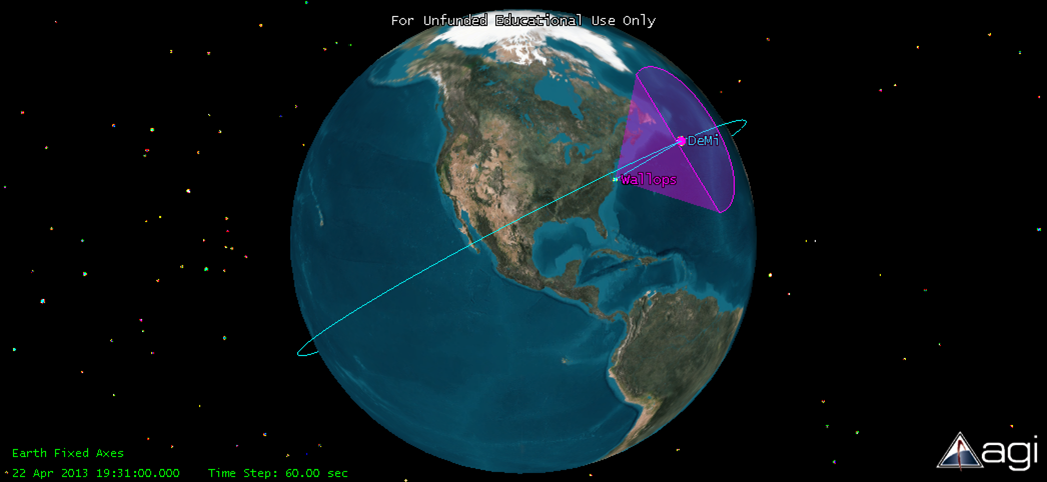
\includegraphics[scale=0.8]{images/ADCS_STK.png}
				\caption{Ground access STK model}
				\label{fig:ADCS_STK}
			\end{figure}
			
			The simulation is run over the course of a day. There are a total of 5 access opportunities of about 9 minutes each. The total ground station access time per day is about 45 minutes. The exact access duration varies with each orbit. 
		
			\subsubsection{Summary of Budgets}
			
			The mass, power, and volume budgets of the ADCS system are presented in Table~\ref{tab:ADCS_budget}
		% Table generated by Excel2LaTeX from sheet 'Sheet4'
\begin{table}[htbp]
  \centering
  \caption{ADCS budgets}
    \begin{tabular}{|r|r|r|r|}
    \hline
    \textbf{Component} & \textbf{Volume} & \textbf{Mass} & \textbf{Power} \bigstrut\\
    \hline
    IMU/Magnetometer & 4.49 $cm^3$ & 0.016 kg & 0.21 W \bigstrut\\
    \hline
    Sun sensors & 6.530 $cm^3$ & 0.02 kg & 0.25 W \bigstrut\\
    \hline
    Torque coils & 58.32 $cm^3$ & 0.52 kg & 1.35 W \bigstrut\\
    \hline
    Interface board & 248.0 $cm^3$ & 0.17 kg & -- \bigstrut\\
    \hline
    \multicolumn{1}{r}{} & \multicolumn{1}{r}{} & \multicolumn{1}{r}{} & \multicolumn{1}{r}{} \bigstrut\\
    \hline
    Total ADCS system (with margin) & 318 $cm^3$ (0.318 U) & 0.73 kg & 1.81 W \bigstrut\\
    \hline
    \end{tabular}%
  \label{tab:ADCS_budget}%
\end{table}%


			\subsubsection{Risks}
			The main design risk in the ADCS system is the pointing stability requirement and the mass and power budget. As previously mentioned, the stability of the satellite will need to be < 0.08$^o$/s for payload science operation of capturing light from a star. The sensors and actuators are expected to provide this performance based on the survey of past CubeSat missions. However, more analysis through simulation and testing will need to be implemented to determine the exact performance of the system. The second risk is due to the narrow margin on the power budget of the whole system. To compensate for this, the mass of the torque coils is higher than previously expected. More iterations will be needed to determine the optimal power consumption and mass of the torque coils. 
			\subsubsection{Future Work}
			The main future work of the ADCS system is to simulate the flight condition through with external disturbance torques at each position on orbit. The next step would be to create a control loop that takes these environmental torques as inputs to compute the needed magnetic moment of each of the 3 torque coils. 
		\subsection{Thermal}
		\subsection{Structure}
\section{Conclusion}
		\subsection{Risk Analysis}
		\subsection{Future Work}
\section{Acknowledgment}
	
	
%%%%%%%%%%%%%%%%%%%%%%%%%%%%%%%%%%%%%%%%%%%%%%%%%%%%%%
% APPENDICES

\newpage
\appendix
\section{\\Requirements} \label{app:requirements}
Requirements go here.

\newpage
\section{\\Link Budgets} \label{app:link_budgets}

\begin{figure}[ht]
\centering 
\caption{Uplink Budget}
\includegraphics[width=8in]{Uplink_Budget.pdf}
\end{figure}

\begin{figure}[ht]
\centering 
\caption{Downlink Budget}
\includegraphics[width=8in]{Downlink_Budget.pdf}
\end{figure}


\newpage

%%%%%%%%%%%%%%%%%%%%%%%%%%%%%%%%%%%%%%%%%%%%%%%%%%%%%%
% REFERENCES
\begin{thebibliography}{9}

%%%%%%%%%%%%%%%%%%%%%%%%%%%%%%%%%%%%%%%%%%%%%%%%%%%%%%
% REFERENCES



%%% PAYLOAD



%%% POWER

\bibitem{CS image}
Image from Clyde Space.  URL \url{http://www.clyde-space.com/cubesat_shop/solar_panels_-_deployable}, (visited May 05, 2013).

\bibitem{libertad-1} (2012).  ``CubeSat Kit -- In Space.''  URL \url{http://www.cubesatkit.com/content/space.html}, (visited May 05, 2013).

\bibitem{EPS manual} Strain, A, (February 14, 2011).  ``User Manual: CubeSat 3U Electronic Power System.'' URL \url{http://www.clyde-space.com/documents/2471}, (visited May 05, 2013).

\bibitem{PDM manual} Worrall, K, (March 14, 2011).  ``CubeSat Power Distribution Module User Manual.'' URL \url{http://www.clyde-space.com/documents/2560}, (visited May 05, 2013).

\bibitem{Battery manual} McLaren, V, (April 28 2010).  ``User Manual: Standalone 30Wh Battery.''  URL \url{http://www.clyde-space.com/documents/1902}, (visited May 05, 2013).

\bibitem{Solar panel datasheet} (March 16 2012). ``CubeSat Solar Panels.''  URL \url{http://www.clyde-space.com/documents/2625}, (visited May 05, 2013).

%%% COMMUNICATIONS

\bibitem{DICE}
``DICE (Dynamic Ionosphere CubeSat Experiment), DICE-1 and DICE-2'', eoPortal, \url{https://directory.eoportal.org/web/eoportal/satellite-missions/d/dice}, Accessed 4/2013.

\bibitem{antenna}
``JPL LMRST Antenna Deployment Test'', \url{http://www.youtube.com/watch?v=DSvHKzM8scc}, Accessed 4/2013.

\bibitem{ITU-R}
``ITU-R P.676-9'', \url{http://www.itu.int/dms_pubrec/itu-r/rec/p/R-REC-P.676-9-201202-I!!PDF-E.pdf}, Accessed 4/2013.

\bibitem{SMAD}
Wertz, James, \emph{Space Mission Engineering: The New SMAD}, Microcosm Press, Hawthorne, CA, 2011.

\bibitem{pozar}
Pozar, David M., \emph{Microwave and RF Design of Wireless Systems}, Wiley, New York City, NY, 2001.

%%% AVIONICS

\bibitem{avionics_clyde_space}
Clyde Space. CubeSat Shop. [Online]. \url{http://www.clyde-space.com/cubesat_shop/obdh/364_mission-interface-computer-grande-em}, visited May 5, 2013. 

%%% ADCS

%%% THERMAL

%%% STRUCTURES

%%% TO BE SORTED

%\bibitem{kim00}
   %Kim. (2000).
  %\emph{\ Simulation Study of A Low-Low Satellite-to-Satellite Tracking Mission}. (Doctoral dissertation)
  %The University of Texas at Austin, TX.

\end{thebibliography}

\end{document}

